% Options for packages loaded elsewhere
\PassOptionsToPackage{unicode}{hyperref}
\PassOptionsToPackage{hyphens}{url}
%
\documentclass[
  12pt,
]{book}
\usepackage{amsmath,amssymb}
\usepackage{lmodern}
\usepackage{setspace}
\usepackage{iftex}
\ifPDFTeX
  \usepackage[T1]{fontenc}
  \usepackage[utf8]{inputenc}
  \usepackage{textcomp} % provide euro and other symbols
\else % if luatex or xetex
  \usepackage{unicode-math}
  \defaultfontfeatures{Scale=MatchLowercase}
  \defaultfontfeatures[\rmfamily]{Ligatures=TeX,Scale=1}
\fi
% Use upquote if available, for straight quotes in verbatim environments
\IfFileExists{upquote.sty}{\usepackage{upquote}}{}
\IfFileExists{microtype.sty}{% use microtype if available
  \usepackage[]{microtype}
  \UseMicrotypeSet[protrusion]{basicmath} % disable protrusion for tt fonts
}{}
\makeatletter
\@ifundefined{KOMAClassName}{% if non-KOMA class
  \IfFileExists{parskip.sty}{%
    \usepackage{parskip}
  }{% else
    \setlength{\parindent}{0pt}
    \setlength{\parskip}{6pt plus 2pt minus 1pt}}
}{% if KOMA class
  \KOMAoptions{parskip=half}}
\makeatother
\usepackage{xcolor}
\IfFileExists{xurl.sty}{\usepackage{xurl}}{} % add URL line breaks if available
\IfFileExists{bookmark.sty}{\usepackage{bookmark}}{\usepackage{hyperref}}
\hypersetup{
  pdftitle={Bayesian Inference for Species Distribution Modelling with Gaussian Processes},
  hidelinks,
  pdfcreator={LaTeX via pandoc}}
\urlstyle{same} % disable monospaced font for URLs
\usepackage[left=1in, right=1in, top=1in, bottom=1in]{geometry}
\usepackage{longtable,booktabs,array}
\usepackage{calc} % for calculating minipage widths
% Correct order of tables after \paragraph or \subparagraph
\usepackage{etoolbox}
\makeatletter
\patchcmd\longtable{\par}{\if@noskipsec\mbox{}\fi\par}{}{}
\makeatother
% Allow footnotes in longtable head/foot
\IfFileExists{footnotehyper.sty}{\usepackage{footnotehyper}}{\usepackage{footnote}}
\makesavenoteenv{longtable}
\usepackage{graphicx}
\makeatletter
\def\maxwidth{\ifdim\Gin@nat@width>\linewidth\linewidth\else\Gin@nat@width\fi}
\def\maxheight{\ifdim\Gin@nat@height>\textheight\textheight\else\Gin@nat@height\fi}
\makeatother
% Scale images if necessary, so that they will not overflow the page
% margins by default, and it is still possible to overwrite the defaults
% using explicit options in \includegraphics[width, height, ...]{}
\setkeys{Gin}{width=\maxwidth,height=\maxheight,keepaspectratio}
% Set default figure placement to htbp
\makeatletter
\def\fps@figure{htbp}
\makeatother
\setlength{\emergencystretch}{3em} % prevent overfull lines
\providecommand{\tightlist}{%
  \setlength{\itemsep}{0pt}\setlength{\parskip}{0pt}}
\setcounter{secnumdepth}{5}
\usepackage{booktabs}
\pagestyle{plain}
\ifLuaTeX
  \usepackage{selnolig}  % disable illegal ligatures
\fi
\usepackage[]{natbib}
\bibliographystyle{apalike}

\title{Bayesian Inference for Species Distribution Modelling with Gaussian Processes}
\usepackage{etoolbox}
\makeatletter
\providecommand{\subtitle}[1]{% add subtitle to \maketitle
  \apptocmd{\@title}{\par {\large #1 \par}}{}{}
}
\makeatother
\subtitle{Isaac William Caruso}
\author{Amherst College\\
Department of Computer Science}
\date{2021-03-30}

\usepackage{amsthm}
\newtheorem{theorem}{Theorem}[chapter]
\newtheorem{lemma}{Lemma}[chapter]
\newtheorem{corollary}{Corollary}[chapter]
\newtheorem{proposition}{Proposition}[chapter]
\newtheorem{conjecture}{Conjecture}[chapter]
\theoremstyle{definition}
\newtheorem{definition}{Definition}[chapter]
\theoremstyle{definition}
\newtheorem{example}{Example}[chapter]
\theoremstyle{definition}
\newtheorem{exercise}{Exercise}[chapter]
\theoremstyle{remark}
\newtheorem*{remark}{Remark}
\newtheorem*{solution}{Solution}
\begin{document}
\maketitle

{
\setcounter{tocdepth}{1}
\tableofcontents
}
\setstretch{1.7}
\hypertarget{probability-bayes-theorem-and-bayesian-inference}{%
\chapter{Probability, Bayes' theorem, and Bayesian inference}\label{probability-bayes-theorem-and-bayesian-inference}}

The objective of this chapter is to provide an introduction and brief summary of the probability terms and concepts necessary for conceptualizing and approaching Bayesian inference.
Simply put, Bayesian inference is a statistical technique for iteratively updating a probability quantity of interest upon the observation of data.
Specifically, the statistical technique Bayesian inference relies on is known as Bayes' theorem and the probability quantity of interest is most often a probability density function, though in introductory examples is oftentimes a single value.
Before embarking on this exposition of Bayesian statistics, one must first gain a basic appreciation for a few key elements of probability theory which will provide us with the foundational terms to discuss Bayesian inference and its applications in the broad field of machine learning---random variables and probability functions.
A brief discussion of random variables will naturally lead to the introduction of cumulative distribution functions and probability functions/ distributions.
An understanding of probability functions will provide the fundamental terminology necessary for introducing a discussion of the concepts expected value and conditional probability.
This chapter will then conclude by introducing Bayes' theorem and Bayesian inference in demonstrating the steps for performing a simple Bayesian update.

\hypertarget{random-variables}{%
\section{Random Variables}\label{random-variables}}

Imagine for a moment you are tossing a coin.
There are many experiments you could perform by tossing a coin, but for the sake of simplicity let us consider our quantity of interest to be the number of times our coin lands on a tails.
It is clear that the number of tails, the outcome of our experiment, is dependent on the eventual realization of some random (stochastic) process, or at the very least not clearly deterministic.
In countless scenarios like the coin toss experiment, random variables provide a convenient and uniform terminology for discussing sample spaces and their connection to some sequence of observations that is the data.
In essence, a random variable is a variable whose value is dependent on the outcome(s) of a stochastic phenomenon.
A random variable is commonly expressed as \(X\), and a realized value of \(X\) is \(x\).

In the canonical example of tossing a coin, where the data is some sequence of coin tosses \([H, T, T, …]\), we could define a random variable \(X\) to be the number of tails.
In this toy example, as noted above, the realized value of \(X\), is dependent on the outcome(s) of a random event---a coin toss.
In the case of tossing a coin twice consecutively, \(X\)---the number of tails observations---has three possible realized states, \(x\), depending on the outcome of this stochastic experiment: \(x = 0\), \(x = 1\), or \(x = 2\).
Additionally, assuming the coin is a fair coin the probability that our random variable \(X\) is realized as \(x\), some real number of tails, can be assigned to each possible overall outcome of this coin toss experiment as represented in Table \ref{tab:rv}

\begin{table}[!h]

\caption{\label{tab:rv}P(X = x) for two tosses}
\centering
\begin{tabular}[t]{rr}
\toprule
x & P(X = x)\\
\midrule
0 & 0.25\\
1 & 0.50\\
2 & 0.25\\
\bottomrule
\end{tabular}
\end{table}

In reality, this is an example of a specific type of random variable known as a discrete random variable.
Discrete random variables can, as their name implies, only assume discrete values.
To the contrary, continuous random variables and mixed random variables are useful for describing sample spaces with continuous and mixed outcomes, respectively.
For example, a continuous random variable may be used to describe an experiment measuring blossoming heights of flowers, where the data is a sequence of observations of heights at which different flowers blossomed.
In this case, the outcome of our blossoming experiment is an infinite number of real values that is properly represented in a continuous random variable.

\hypertarget{cumulative-distribution-functions}{%
\section{Cumulative Distribution Functions}\label{cumulative-distribution-functions}}

The concept of a distribution follows intuitively from our previous discussion of random variables.
In the previous example we represented the probability of various outcomes of a coin toss experiment in a tabular format.
Another way to represent this distribution of probabilities is as a cumulative distribution function:

\begin{definition}[Cumulative distribution function 'CDF']
\protect\hypertarget{def:cdf}{}{\label{def:cdf} \iffalse (Cumulative distribution function `CDF') \fi{} }\emph{The cumulative distribution function is defined as a function where \(F_{X}\in[0, 1]\):}
\[F_{X}(x)=P(X≤x)\]
\end{definition}

As the name implies, the cumulative distribution function simply represents the probability that a random variable \(X\) is realized to be less than or equal to \(x\) for each possible input value of \(x\).
Figure \ref{fig:cdfimg} depicts a graphical representation of the CDF for our coin tossing experiment.

\begin{figure}

{\centering 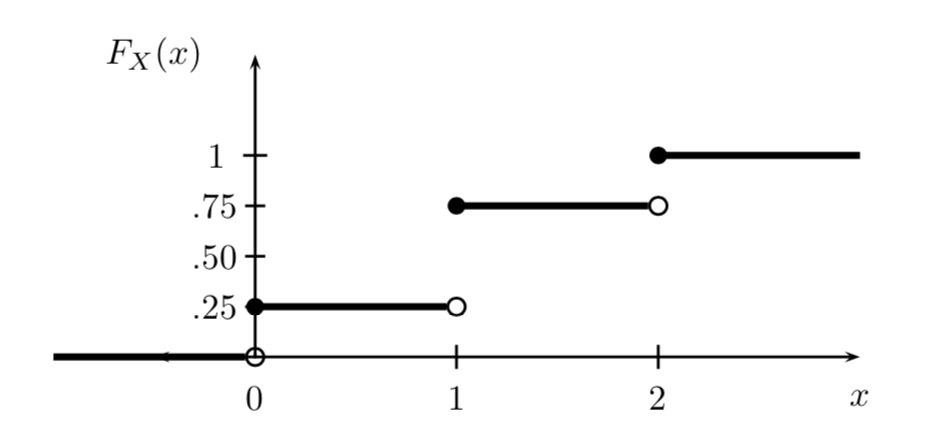
\includegraphics[width=0.7\linewidth]{./images/cdf} 

}

\caption{CDF for tossing a coin twice (from All of Stats, should I make my own?)}\label{fig:cdfimg}
\end{figure}

Here, for every value of \(x\)---the number of tails in two coin tosses---the probability that \(X\) is equal to or less than this value is represented.
In this discrete example, we see that our CDF is represented by several non-decreasing discrete lines defined for all \(x\).
In the example of a continuous random variable, this function is a continuous, non-decreasing distribution also defined for all \(x\).

\hypertarget{probability-mass-and-density-functions}{%
\section{Probability Mass and Density Functions}\label{probability-mass-and-density-functions}}

Now that we have a basic understanding of random variables and their association with the CDF, we can begin discussing probability functions for both continuous and discrete random variables.
Broadly speaking, the probability mass function and probability density function are two methods for calculating a probability over a sample space, which find their use with discrete and continuous random variables respectively.

In the discrete setting, a probability mass function yields the probability of an outcome for every possible outcome in any given discrete schema.
To reiterate the previous discussion of discrete versus continuous random variables, a random variable \(X\) is considered discrete ``if it takes countably many values \(\{x_{1}, x_{2}, …\}\)'' \citep{Wasserman2004}.
In this case, a definition for the probability mass function follows:

\begin{definition}[Probability mass function 'PMF']
\protect\hypertarget{def:pmf}{}{\label{def:pmf} \iffalse (Probability mass function `PMF') \fi{} }\emph{The probability function for a discrete random variable \(X\)---the probability mass function for \(X\)---is defined as a function}
\[F_{X}(x)=P(X=x)\]
\end{definition}

Here, the PMF has a few key attributes.
Namely \(P(X=x)>0\) for every \(x\) in the sample space of \(X (x \in S_{X})\), and \(\sum_{x \in S_{X}}f(x)=1\).
With these features in mind, the probability mass function of \(X\) follows logically from the cumulative distribution function of \(X\) insofar as the CDF is the sum of the PMF for all \(x_{i}≤x\).
This relationship in the discrete scenario between the PMF and CDF can be expressed formally as: \[F_{X}(x)=P(X≤x)=\sum_{x_i≤x}f_{X}(x_{i})\]

In the continuous setting where these attributes no longer hold, a probability density function (PDF) is instead used to represent probability of \(x\) for all \(x \in S_X\).
In the case where the random variable \(X\) is continuous, a PDF is defined as follows:

\begin{definition}[Probability density function 'PDF']
\protect\hypertarget{def:pdf}{}{\label{def:pdf} \iffalse (Probability density function `PDF') \fi{} }\emph{The probability function for a continuous random variable \(X\)---the probability density function for \(X\)---is defined as a function \(f(x)\) where \(a\) and \(b\) are two real numbers and every \(a ≤ b\), so}
\[P(a<X<b)=\int_{a}^{b}f_X(x)dx\]
\end{definition}

In other words, the probability that the realized value \(x\) of our continuous random variable \(X\) is between two numbers \(a\) and \(b\) is equal to the integral of the probability density function of \(x\) from \(x = a\) to \(x = b\).
This formalization of the PDF \(f_X(x)\) allows a natural comparison to be drawn to the CDF \(F_X(x)\) of a continuous random variable \(X\), that is:

\[F_X(x)=\int_{-\infty}^{x}f_X(x)dx\]

Specifically, this implies that \(F'_X(x)=f_X(x)\) for all differentiable points in \(F_X\).
In plain English this signifies that the derivative of the CDF is the PDF, in all cases involving a continuous random variable.

Probability density and mass functions come in a wide variety of forms, each with their own properties and methodologies for defining their shape and characteristics.
Some are useful for defining binary data, others are useful for defining arbitrarily large sample spaces with any number of localized concentrations of density.
Still others boast properties, such as being closed under conditioning and marginalization, that make them useful for specific statistical applications.
Figure \ref{fig:distributions} displays some of the most common continuous and discrete probability distributions.

\begin{figure}

{\centering 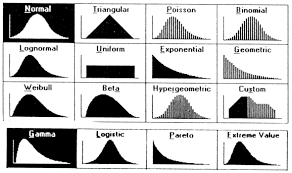
\includegraphics[width=0.7\linewidth]{./images/distributions} 

}

\caption{Common probability distributions}\label{fig:distributions}
\end{figure}

\hypertarget{expectation}{%
\section{Expectation}\label{expectation}}

One of the final core statistical concepts necessary to approach Bayesian statistics on sure footing is the idea of expectation or expected value.
Simply put, the expectation of a random variable \(X\) is the average value of \(X\).

\begin{definition}[Expectation '$E$']
\protect\hypertarget{def:e}{}{\label{def:e} \iffalse (Expectation `\(E\)') \fi{} }\emph{The expectation, expected value, or mean of a random variable X is}
\[E(X)=EX=\begin{cases}\sum_{x}xf(x) & \textrm{if }X\textrm{ is discrete}\\\int{xf(x)dx} & \textrm{if }X\textrm{ is continuous}\end{cases}\]
\end{definition}

While on first glance the expectation may appear unfamiliar and dissimilar to the common understanding of a mean, key characteristics of probability distributions will foster an intuitive understanding of their similarities.
To return to a familiar example, consider a random variable \(X\) to represent the number of tails in 6 coin tosses. Figure \ref{fig:binom} depicts the PMF for \(X\) using the binomial distribution, which represents the probability of observing a specific number of successes in a success-failure experiment.

\begin{figure}

{\centering 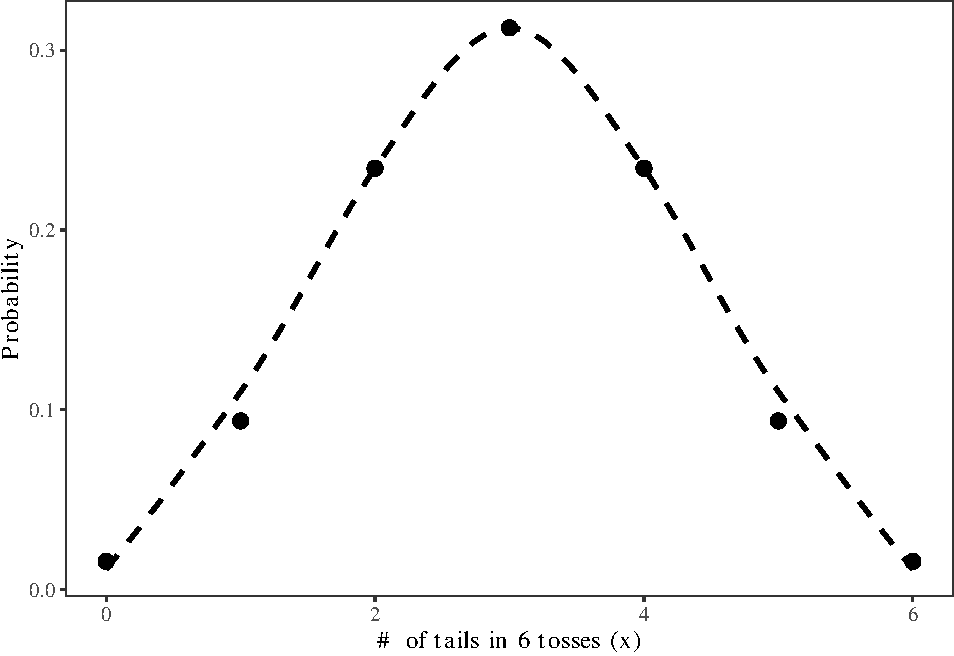
\includegraphics[width=0.7\linewidth]{manuscript_files/figure-latex/binom-1} 

}

\caption{The binomial probability mass function for the 6 trial coin toss experiment}\label{fig:binom}
\end{figure}

In this case, the x-axis represents each particular outcome (\(x\)) of \(X\) and the y-axis is the relative probability of that outcome. Table \ref{tab:bino} presents the output of the binomial PMF for every \(x \in X\).

\begin{table}[!h]

\caption{\label{tab:bino}P(X = x) for six tosses}
\centering
\begin{tabular}[t]{rr}
\toprule
x & y\\
\midrule
0 & 0.016\\
1 & 0.094\\
2 & 0.234\\
3 & 0.312\\
4 & 0.234\\
5 & 0.094\\
6 & 0.016\\
\bottomrule
\end{tabular}
\end{table}

Computing \(EX\) given the values in this table is demonstrated using the discrete case of Definition \ref{def:e} in Example \ref{exm:coin}.

\begin{example}
\protect\hypertarget{exm:coin}{}{\label{exm:coin} }The expected value of a discrete random variable \(X \sim B(6, 0.5)\), which represents the number of tails in 6 coin tosses and has a binomial distribution, is calculated as follows:
\[\begin{split}
E(X) & = \sum_{x}xf(x) \\
  & =  (0*0.16)+(1*0.094)+(2*0.234)+(3*0.312)+(4*0.234)+(5*0.094)+(6*0.016)\\
  & = 3
\end{split}\]
\end{example}

Naturally, the expected value of \(X\) is 3 in Example \ref{exm:coin}.
Importantly, while in this case \(EX\) corresponds well to the peak in the PMF for this experiment this should not be assumed to be the case unilaterally, as the same expectation would result from any distribution symmetrical about \(x=3\).
While surfically the expected value of a random variable may appear to be a trivial reframing of the calculating of a mean, it is crucial to note that expectation is calculated using the relative probability of \(x\) in lieu of the number of observations in the sample space.
In the continuous case, this is the property that makes computing the expectation possible.
To summarize, in the field of probability the expected value provides a crucial, unifying term for the characterization of probability distributions.
This term will prove useful in many situaions, including normalization in the context of Bayes' theorem.

\hypertarget{conditional-probability}{%
\section{Conditional Probability}\label{conditional-probability}}

Conditional probability provides a uniform, comprehensible format for considering the probability of events which are dependent on the outcome of a different event. Conditional probability, as presented in Definition \ref{def:condprob}, requires only that the event on which some other event depends has some nonzero probability of occuring.

\begin{definition}[Conditional Probability]
\protect\hypertarget{def:condprob}{}{\label{def:condprob} \iffalse (Conditional Probability) \fi{} }\emph{Assuming \(P(B)>0\),}
\[P(A|B)=\frac{P(AB)}{P(B)}\]
\end{definition}

Conditional probability asserts that the probability of event A occuring given that event B occurs is equivalent to the probability of both A and B occuring divided by the probability that B occurs. Example \ref{exm:condprobe} explains how to use conditional probability to calculate the probability of drawing an ace from a deck given I drew a king. While it may seem logical to conclude that \(P(A|B)=P(B|A)\), this is not the case generally speaking.
For example, the probability that I can swim given that I am in the water is clearly not the same as the probability that I am in the water given that I can swim.

\begin{example}
\protect\hypertarget{exm:condprobe}{}{\label{exm:condprobe} }Conditional probability can be used to determine the probability of drawing an ace from a standard deck of cards without replacement, given I first drew a king from that deck. This scenario can be represented as:
\[A = \textrm{Draws ace, } P(A) = 4/51\]
\[B = \textrm{Draws king, } P(B) = 4/52\]
\[\begin{split}
P(ace|king) = P(A|B) & = \frac{P(AB)}{P(B)} \\
  & = \frac{\frac{4}{51}\frac{4}{52}}{\frac{4}{52}} \\
  & = \frac{4}{663} = 0.00603
\end{split}\]
\end{example}

\hypertarget{bayes-theorem}{%
\section{Bayes' Theorem}\label{bayes-theorem}}

Under construction\ldots{} \citep{Kotta2019}

\hypertarget{bayesian-inference}{%
\section{Bayesian Inference}\label{bayesian-inference}}

\hypertarget{approximation-algorithms-for-inference-on-complex-systems}{%
\chapter{Approximation algorithms for inference on complex systems}\label{approximation-algorithms-for-inference-on-complex-systems}}

\hypertarget{modern-bayesian-inference-with-stan}{%
\chapter{Modern Bayesian inference with STAN}\label{modern-bayesian-inference-with-stan}}

\hypertarget{bayesian-applications-in-biology-hybrid-species-distribution-modelling-with-gaussian-processes}{%
\chapter{Bayesian applications in Biology: Hybrid species distribution modelling with gaussian processes}\label{bayesian-applications-in-biology-hybrid-species-distribution-modelling-with-gaussian-processes}}

  \bibliography{references.bib,packages.bib}

\end{document}
